\documentclass[runningheads]{llncs}
%
\usepackage{graphicx}
% Used for displaying a sample figure. If possible, figure files should
% be included in EPS format.
%
% If you use the hyperref package, please uncomment the following line
% to display URLs in blue roman font according to Springer's eBook style:
% \renewcommand\UrlFont{\color{blue}\rmfamily}

\begin{document}
%
\title{The Standard Vessel Capacity Model:\\ A Convex Polyhedron Representation of\\ Container Vessel Capacity\thanks{This research is supported by the Danish Maritime Fund grant no. 2016-064.}}
%
\titlerunning{The Standard Vessel Capacity Model}
% If the paper title is too long for the running head, you can set
% an abbreviated paper title here
%
\author{Mai Lise Ajspur\inst{1} \and
Rune M{\o}ller Jensen\inst{1}}
%
\authorrunning{M.L. Ajspur and R.M. Jensen}
% First names are abbreviated in the running head.
% If there are more than two authors, 'et al.' is used.
%
\institute{The IT University of Copenhagen, Rued Langaards Vej 7, 2300 Copeenhagen S, Denmark}
\email{ajspur,rmj@itu.dk}
%
\maketitle              % typeset the header of the contribution
%
\begin{abstract}
The abstract should briefly summarize the contents of the paper in
15--250 words.

\keywords{First keyword  \and Second keyword \and Another keyword.}
\end{abstract}

\section{Introduction}
Container liner shipping is a major driver of the world economy\cite{TE13}. There are more than 5000 container vessels in the world today \cite{RMT16}, mostly sailing on cyclic services with published fixed weekly schedules and freight rates. Liner shipping companies adjust their service networks and fleet over the year to fit seasonal trends and long-term developments in the world economy, but they seldom make fleet and network changes due to current cargo on the network and known bookings (Mikkel persal communic). For that reason, it is a central business objective to maximize the utilization of the service network. Any free capacity in the network is an opportunity for business.

In this aspect, the container shipping and airline industry is similar. It is all about filling the slots on the vessels. A closer inspection shows, however, that the domains are rather different. Air planes are usually completely emptied at each destination, and an empty seat in most cases means that the plane can fit one more passenger. This has enabled the airlines to apply advanced revenue management methods such as dynamic pricing and over-booking to maximize the utilization of the planes.

Previous work has studied how to apply revenue management methods in the liner shipping industry (e.g., Sebastian), but it has turned out to be challenging in practice. A major obstacle is how to compute the free capacity of a container vessel. It is not simply the number of vacant slots on the vessel. A large number of local and global constraints may cause slots to be impossible to use including: stacking limitations due to different length, height, power need (reefer containers), and dangerous content of containers; limited volume, weight, and securing capacity of container stacks; vessel hydrostatics like stability requirements and stress force limitations; containers blocking each other due to different port of discharge; capacity preserving stowage patterns; and work balancing of quay cranes (see Section~\ref{} for details).

It is recognized by leading economists that this problem blocks a paradigm change in liner shipping. According to Martin Stopford the ability to match spare capacity to cargo in need of transportation on the fly would allow the "Uberisation" of the freight business \cite{EApril18}. Today, the higher sales and cargo flow functions in liner shipping companies are unable to make these matchings. The spare capacity of a container vessel is often simply calculated as its maximum volume, weight, and reefer container capacity subtracted the capacity taken up by on board cargo without consideration of losses due stowage restrictions and rules (personal communication Mikkel M). This can cause great over-estimates of the free capacity of the vessels (delgado thesis).

In the last two decades, a number of automated stowage planning methods have been published (e.g., roach, kim kang, ambrosino, pacino (ICLL 11, all late publications). The input to these methods is the arrival condition of the vessel and a list of containers to load and the output is a stowage plan. As such, these methods are unable to compute the spare capacity of the vessel, since the containers to load are assumed to be known. Several of the contributions, though, apply optimization models, where the containers to load can act as decision variables rather than constants (e.g. ambrosino Aberlto pacino, etc). There is also recent work on maximizing the utilization of a vessel on a given circular service route with limitations on expected cargo (alberto, pacino). 

These models can be used to compute the spare capacity of a vessel. In practice, though, they can be challenging to apply in higher functions such as sales and cargo flow. The stowage planning problem is NP-hard (org. NP hardness proof), even in its various abstract versions (our NP-hardness proof). This means that the stowage optimization models can take long time to solve, which also happens in practice (e.g., pacino 11). Since it can take more than five hours to generate a stowage plan manually, this is an acceptable evil in stowage planning. In higher functions, on the other hand, capacity models can be parts of larger optimization models which require that they are scalable. For instance, in capacity and uptake management, a cargo flow network could be used to match cargo demand with spare capacity. In such a network over a handful of weeks of a major trade line, there would be thousands of edges representing voyage legs, and each of these would be associated with a capacity model. 

To address this challenge, this paper introduces the {\em standard vessel capacity model} (SVCM). The SVCM is based on several insights from our previous work on stowage planning optimization. First, a lot of the complexity and inaccessibility of these models stem from the fact that data describing container vessels is spatially misaligned. To clear this, the SVCM interpolates vessel data to align with the endpoints of each bay. Second, stowage optimization models have many details that can be abstracted away in capacity calculations. To this end, the granularity of SVCMs can be adjusted. At the finest level, each bay form a {\em section}. At coarser levels, adjacent sections are merged. Third but not least, our previous studies of vessel hydrostatics (cite ICCL on hydro model) show that these can be accurately approximated by linear functions within a displacement interval. Our industrial continuation of this work has shown that surprisingly many highly complex aspects of stowage planning such as the limited forces in lashing gear either can be linearly expressed or can be approximated with convex step-wise linear functions (cite optivation). The intractable elements of stowage planning include separation rules of containers with dangerous goods and the fact that quay cranes only can discharge containers from the top of stacks (org. NP hardness proof). In more abstract capacity models, though, it may be possible to express some of these combinatorial aspects as linear trade-offs. In other words, it is worthwhile to investigate whether accurate polyhedron approximations to vessel capacity constraints can be formulated. If this is the case, they can be embedded in larger optimization frameworks as linear programs (LPs). This is attractive due to the polynomial complexity of LPs. The SVCM is a step in this direction. To our knowledge, it introduces the first linear approximation of hydrostatic equilibrium and metacentric height that is independent of vessel displacement. It further includes a number of non-trivial examples of linear trade-offs in stowage planning.

Our results show ...

The remainder of this paper is organized as follows. ...

\section{Problem Formulation}

Container vessels mainly transport ISO containers with the dominating lengths 20', 40', and 45'. The containers are usually 8' wide. There are two common heights: standard 8'6" (DC) and high-cube 9'6" (HC). Containers have corner fittings that allow them to be stacked upto 10 high (). Figure~\ref{fig:container_intermediate_fittings} shows the position of corner fittings (left) and the stowage rules they cause (right): no 20' on 40' or 45' and no 40' on 45'.      
\begin{figure}[h!]
\centering 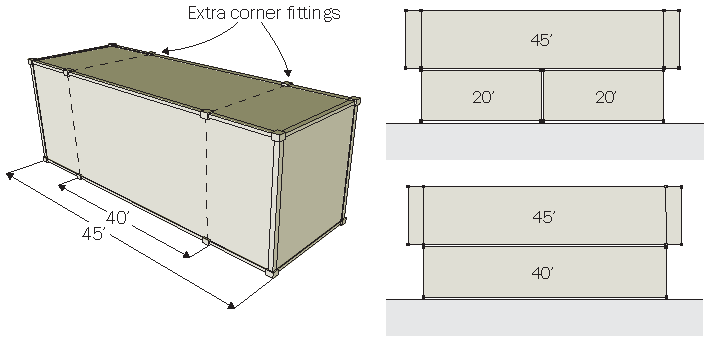
\includegraphics[scale=0.7]{figures/2_3}
\caption{Corner fittings and Intermediate fittings.\label{fig:container_intermediate_fittings}}
\end{figure}
The cargo space of a container vessel is divided into \textit{bays} that each consists of a grid of \emph{cells} (see Figure~\ref{fig:vessel}). Each cell is divided into a fore and aft \emph{slot} and can accordingly hold one 40' container or two 20' containers. Some cells have power plugs allowing for \emph{reefer} containers to be refrigerated as required. Each bay is divided into stowage areas above and under hatch covers that separate on deck and below deck cells. We refer to these as {\em locations}.
\begin{figure}[h!]
	\centering
		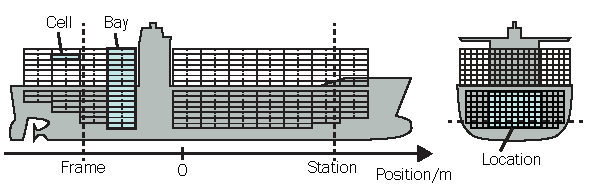
\includegraphics{figures/vessel2.pdf}
	\caption{(a) Vessel structure and reference points seen on a longitudinal intersection X, and (b) on a transversal intersection.}
	\label{fig:vessel}
\end{figure}

The are significant resulting gravity and boyancy forces acting on a vessel in typical load conditions as illustrated in Figure~\ref{fig:split_vessel}. This causes longitudinal shear forces (SF) and bending moments (BM) and transversal torsion moments (TM). These must be within limits given by the classification society of the vessel. 
\begin{figure}[h!]
\begin{center}
  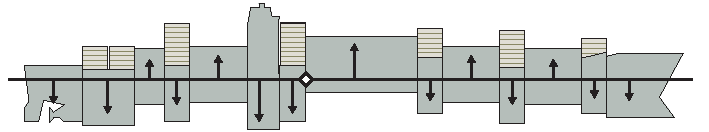
\includegraphics{figures/3_12}
\end{center}
\caption{Example of the effects of uneven distribution of weights and buoyancy forces along different sections of a container vessel.}
\label{fig:split_vessel}
\end{figure}

Figure~\ref{fig:stability} (a) illustrates the position of the vertical center of gravity ($G$) and  ($B$) when the vessel is upright. When the vessel lists due to an external force such as waves, the center of byoancy moves in the direction of the list (Figure~\ref{fig:stability} (b)). For small angles, a vertical line through the center of boyauncy interscts the center line in a constant position ($M$). If the vertical center of gravity is above $M$, it moves faster in the direction of the tilt than $M$ and the vessel capsizes. The distance between $G$ and $M$ is referred to as $\mathit{GM}$ or metacentric height and classification societies requires a minimum $\mathit{GM}$.
\begin{figure}[h!]
  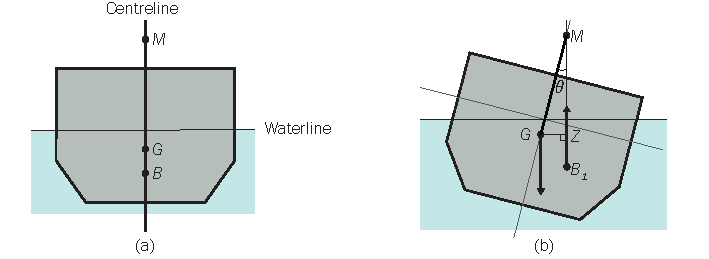
\includegraphics{figures/3_11} 
\caption{ Transversal view of a vessel at even keel (a) and vessel perturbed by a external heeling force (b).}
\label{fig:stability}
\end{figure}

Other seaworthiness requirements include LOS, IMDG, LSHING, stack weights,

\begin{figure}[h!]
  \centering
  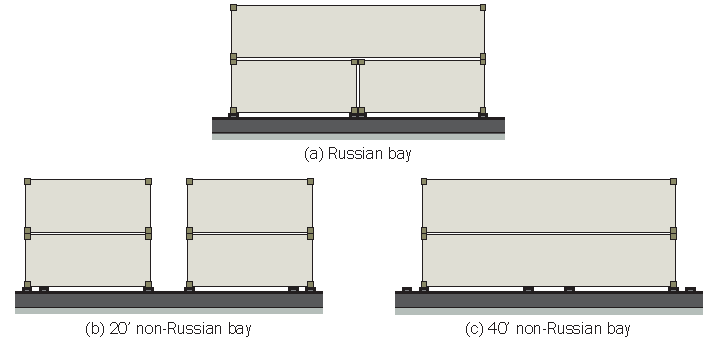
\includegraphics{figures/3_36}
  \caption{The position of 20' and 40' containers in Russian (a) and non-Russian stowage (b) and (c).}\label{fig:OnDeckContainerPlacementInSockets}
\end{figure}

\begin{figure}[h!]
  \centering
  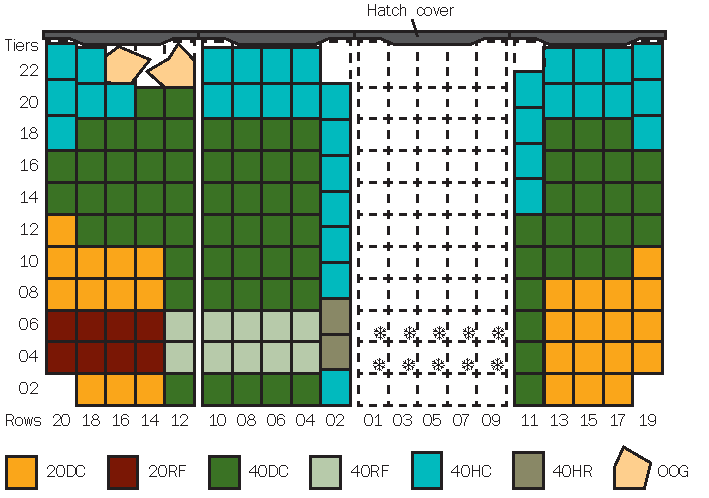
\includegraphics{figures/3_24}
  \caption{Aft view of a typical stowage pattern below deck.}\label{fig:BelowDeckPattern}
\end{figure}


\begin{figure}[h!]
  \centering
  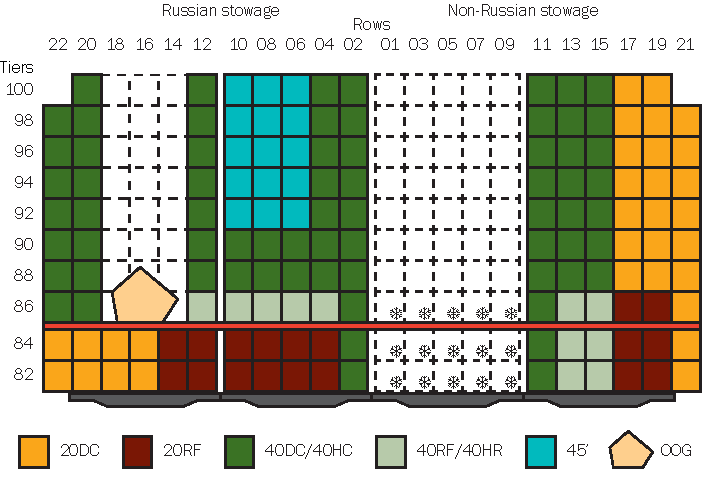
\includegraphics{figures/3_40}
  \caption{Aft view of a typical stowage pattern on deck. The port (even rows) and starboard (odd rows) patterns are for Russian and non-Russian stowage, respectively. The thick red horizontal line between tier 84 and 86 indicates the position of the lashing bridge.}\label{fig:ObjectivesOnDeck}
\end{figure}



The residual capacity of a container vessel. It is not simply the number of vacant slots on the vessel, since slots may be impossible to occupy for a large number of interdependent reasons. First, there are the stacking rules of containers. It is impossible to stack 20’ containers on top of 40’ and 45’ containers due to the lack of support. 45’ containers normally only fit in special 45’ bays or over the lashing bridge on deck and reefer containers that require external power must be placed close to a power supply. There may also be containers with dangerous goods like firework that have to be separated from other such containers. Second, each stack has limited capacity. Below deck the hatches that covers the holds define the maximum height of stacks. Since standard containers are either 8’6’ (DC) or 9’6” (HC), this means that volume may be lost in a stack due to a bad mixture of HC and DC containers. On deck, line-of-sight rules may lead to lost slots in the fore part of the vessel. The bottom sockets also have limited weight capacity, which can cause lost slots due to heavy containers in a stack. Even if neither the volume nor the weight capacity of a stack on deck is exhausted, it may still be unable to hold more containers due to excessive forces in the lashing gear. Open top containers and breakbulk cargo like windmill wings may also cause lost slots. Third, slots may be lost for hydrostatic reasons. If the vertical center of gravity gets too high, the vessel may be in danger of capsizing. Slots may also be lost, because filling them may lead to undesirable longitudinal or transversal weight distributions that break stress limits like shear (SF), bending (BM), and torsion (TM) or lead to suboptimal trim or draft of the vessel. Forth, slots may be lost to avoid that containers block each other. If a container is placed above another container in the same stack destined for an earlier port, it blocks this container and must be restowed. In particular, if a container is placed in hold, it is blocked by any container placed on the hatch of the hold destined for later ports. Fifth, since cargo to load future ports is uncertain, stowage plans apply robustness principles to keep them flexible to future cargo. One is paired block stowage, where the same port of discharge (POD) is chosen for all containers above and below a hatch cover and where the wing blocks of a bay have the same POD to avoid incurring torsion when the containers are unloaded. This principle alone limits the available slots for containers with a particular POD. Finally, sixth the utilization of quay cranes must be maximized to reduce the port stay. Since it is common to use more than six cranes to discharge and load a vessel this means that slots may be lost because using them may uneven the load balance between the cranes      principles to are applied in  

all containers for later         



The longitudinal positions of bays are misaligned with cross-section stations in the Bonjean table that are misaligned with frame positions defining limits of stress forces. All of these data again are misaligned with ballast and fuel tank positions and blocks defining the weight distribution of the empty ship.



\bibliographystyle{splncs04}
\bibliography{references}

\end{document}
